\documentclass[aspectratio=169]{beamer}
\mode<presentation> {
\usetheme{default}
\usecolortheme{dolphin}
}
\usepackage{algorithm,algorithmic}
\usepackage{caption}
\usepackage{multirow}
\usepackage{threeparttable}
\usepackage{graphicx}
\usepackage{parskip}
\usepackage{float}
\usepackage{alphabeta}
\usepackage{multirow,array}
\usepackage{subfig}
\usepackage{amsmath}
\usepackage{amssymb}
\usepackage{mathabx}
\usepackage{caption}
\usepackage{pifont} 
\usepackage{booktabs,tabularx}
\usepackage{tikz}
\usetikzlibrary{shapes,arrows}
\usepackage[table]{xcolor}
\newcolumntype{Y}{>{\raggedright\arraybackslash}X}

\usepackage{tikz}
\usetikzlibrary{arrows.meta,positioning,calc,fit,backgrounds,decorations.pathreplacing, shapes.geometric}
\graphicspath{{figures/}}
\usetikzlibrary{matrix,chains,positioning,decorations.pathreplacing,arrows}

% TikZ Styles - Adjusted font sizes for clarity since bold is removed
\tikzset{
  >=Stealth,
  st/.style={circle,draw,inner sep=0pt,minimum size=6mm, fill=white}, 
  action/.style={circle,fill=black,inner sep=0pt,minimum size=2mm},
  tr/.style={-Stealth, line width=0.8pt},
  lbl/.style={font=\footnotesize},
  block/.style={rectangle, draw, fill=blue!10, rounded corners, minimum height=2em}
}

\newcommand{\E}{\mathbb{E}}
\newcommand{\R}{\mathbb{R}}
\newcommand{\1}{\mathbf{1}}
\newcommand{\loss}{\mathcal{L}}
\newcommand{\X}{\mathcal{X}}
\newcommand{\Y}{\mathcal{Y}}
\newcommand{\D}{\mathcal{D}}
\newcommand{\thetavec}{\boldsymbol{\theta}}
\DeclareMathOperator*{\argmax}{arg\,max}
\DeclareMathOperator*{\argmin}{arg\,min}
\setbeamertemplate{caption}[numbered]
\setbeamertemplate{navigation symbols}{}
\setbeamertemplate{footline}[frame number]

\title{Heterogeneous Agent Model}

\author{Yasuyuki Sawada, Yaolang Zhong}
\institute{University of Tokyo\\
  \small \texttt{\href{mailto:yaolang.zhong@e.u-tokyo.ac.jp}{yaolang.zhong@e.u-tokyo.ac.jp}}}
\date{}

\begin{document}

\begin{frame}
\titlepage  
\end{frame}



\begin{frame}{Recap: Motivation for Machine Learning}
  \begin{itemize}
      \item Dynamic programming faces the curse of dimensionality
      \begin{itemize}
          \item Parameterization problem
          \begin{itemize}
              \item Classical functional forms (linear, polynomials, splines)
              \item Number of basis terms grows rapidly with state dimension
              \item Strong restrictions and poor capture of interactions
          \end{itemize}
          \item Grid / data problem
          \begin{itemize}
              \item Grid-based DP requires $N^d$ state points
              \item Computation and memory grow exponentially
              \item Sparse grids mitigate but do not eliminate the problem
          \end{itemize}
      \end{itemize}
  \end{itemize}
  \end{frame}

  \begin{frame}{How Machine Learning Addresses the Curse of Dimensionality}
    \begin{itemize}
        \item Machine learning relaxes both constraints
        \begin{itemize}
            \item Neural networks for parameterization
            \begin{itemize}
                \item Flexible, high-dimensional function approximation
                \item Captures nonlinearities and interactions
            \end{itemize}
            \item \textcolor{blue}{Stochastic simulation for data collection}
            \begin{itemize}
                \item \textcolor{blue}{Learn from simulated trajectories, not full grids}
                \item \textcolor{blue}{Scales to high-dimensional state spaces}
            \end{itemize}
        \end{itemize}
    \end{itemize}
    \end{frame}

%% ============================================================
%% SECTION: RL Data Management
%% ============================================================

\begin{frame}{RL for Economic Models: Data Generation}
  \begin{itemize}
      \item One observation: $(s, a, r, s')$
        \begin{itemize}
            \item $s$: taken as given
            \item $a$: determined by policy $\sigma_\theta(s)$
            \item $r, s'$: determined by the environment's reward function $R(s, a)$ and transition function $P(s' \mid s, a)$
        \end{itemize}
      \item Policy Evalution (Update $Q_\phi^\sigma$) --- requires $\sigma_\theta$ from Policy Improvement:
        \begin{itemize}
          \item Fixed-point iteration:
          $$Q_\phi^\sigma(\textcolor{blue}{s}, \textcolor{blue}{a}) \leftarrow R(\textcolor{blue}{s},\textcolor{blue}{a}) \;+\; \beta \sum_{\textcolor{blue}{s'}} P(\textcolor{blue}{s'} \mid \textcolor{blue}{s},\textcolor{blue}{a})\, Q_\phi^\sigma\big(\textcolor{blue}{s'}, \sigma_\theta(\textcolor{blue}{s'})\big)$$
          \item Gradient-based update:
          \begin{align*}
            \phi \leftarrow \phi - \alpha \nabla_\phi \underbrace{\left( R(\textcolor{blue}{s},\textcolor{blue}{a}) \;+\; \beta \sum_{\textcolor{blue}{s'}} P(\textcolor{blue}{s'} \mid \textcolor{blue}{s},\textcolor{blue}{a})\, Q_{\bar{\phi}}^\sigma\big(\textcolor{blue}{s'}, \sigma_\theta(\textcolor{blue}{s'})\big) - Q_\phi^\sigma(\textcolor{blue}{s}, \textcolor{blue}{a}) \right)^2}_{\text{Loss}}
          \end{align*}
        \end{itemize}
  \end{itemize}
\end{frame}

\begin{frame}{RL for Economic Models: Q-Learning / Value Iteration}
  \begin{itemize}
      \item One observation: $(s, a, r, s')$
      \item Q-Learning (Update $Q_\phi$) --- self-contained, only $Q_\phi$ needed:
        \begin{itemize}
          \item Fixed-point iteration:
          $$Q_\phi(\textcolor{blue}{s}, \textcolor{blue}{a}) \leftarrow R(\textcolor{blue}{s},\textcolor{blue}{a}) \;+\; \beta \sum_{\textcolor{blue}{s'}} P(\textcolor{blue}{s'} \mid \textcolor{blue}{s},\textcolor{blue}{a})\, \max_{\textcolor{blue}{a'}} Q_\phi(\textcolor{blue}{s'}, \textcolor{blue}{a'})$$
          \item Gradient-based update:
          \begin{align*}
            \phi \leftarrow \phi - \alpha \nabla_\phi \underbrace{\left( R(\textcolor{blue}{s},\textcolor{blue}{a}) + \beta \sum_{\textcolor{blue}{s'}} P(\textcolor{blue}{s'} \mid \textcolor{blue}{s},\textcolor{blue}{a})\, \max_{\textcolor{blue}{a'}} Q_{\bar{\phi}}(\textcolor{blue}{s'}, \textcolor{blue}{a'}) - Q_\phi(\textcolor{blue}{s}, \textcolor{blue}{a}) \right)^2}_{\text{Loss}}
          \end{align*}
        \end{itemize}
  \end{itemize}
\end{frame}

\begin{frame}{RL for Economic Models: Policy Improvement}
  \begin{itemize}
      \item One observation: $(s, a, r, s')$
      \item Policy Improvement (Update $\sigma_\theta$) --- requires $Q_\phi$ from Policy Evaluation:
        \begin{itemize}
          \item Fixed-point iteration:
          $$\sigma_\theta(\textcolor{blue}{s}) \leftarrow \argmax_{\textcolor{blue}{a}} Q_\phi(\textcolor{blue}{s}, \textcolor{blue}{a})$$
          \item Gradient-based update:
          \begin{align*}
            \theta \leftarrow \theta + \alpha \nabla_\theta \underbrace{\log \sigma_\theta(\textcolor{blue}{a} \mid \textcolor{blue}{s}) \cdot A(\textcolor{blue}{s}, \textcolor{blue}{a})}_{\text{Policy Gradient}}
          \end{align*}
          where $A(\textcolor{blue}{s},\textcolor{blue}{a}) = Q_\phi(\textcolor{blue}{s},\textcolor{blue}{a}) - \mathbb{E}_{\textcolor{blue}{a} \sim \sigma_\theta}[Q_\phi(\textcolor{blue}{s},\textcolor{blue}{a})]$ is the advantage
        \end{itemize}
  \end{itemize}
\end{frame}

\begin{frame}{RL for Economic Models: Euler Equation Update}
  \begin{itemize}
      \item One observation: $(s, a, r, s')$ where $a = c$ (consumption), $s = (k, z)$
      \item Euler Equation Residual (Update $c_\theta$) --- self-contained, only $c_\theta$ needed:
        \begin{itemize}
          \item Fixed-point iteration:
          $$u'(c_\theta(\textcolor{blue}{s})) = \beta \sum_{\textcolor{blue}{s'}} P(\textcolor{blue}{s'} \mid \textcolor{blue}{s}, \textcolor{blue}{a})\, \left[ 1 + r(\textcolor{blue}{s'}) - \delta \right] u'(c_\theta(\textcolor{blue}{s'}))$$
          \item Gradient-based update:
          \begin{align*}
            \theta \leftarrow \theta - \alpha \nabla_\theta \underbrace{\left( u'(c_\theta(\textcolor{blue}{s})) - \beta \sum_{\textcolor{blue}{s'}} P(\textcolor{blue}{s'} \mid \textcolor{blue}{s})\, R'(\textcolor{blue}{s'})\, u'(c_\theta(\textcolor{blue}{s'})) \right)^2}_{\text{Euler Residual Loss}}
          \end{align*}
          where $R'(\textcolor{blue}{s'}) = 1 + r(\textcolor{blue}{s'}) - \delta$ is the gross return
        \end{itemize}
  \end{itemize}
\end{frame}

\begin{frame}{State Sampling Methods}
  \begin{itemize}
      \item Updates require samples $(s, a, r, s')$; given $s$, the tuple is determined by $(\sigma_\theta, R, P)$
      \item Three approaches to obtain state $s$:
      \begin{enumerate}
          \item Grid-based (non-stochastic): Deterministic enumeration over $\mathcal{S}$
          \[
          s \in \{s^{(1)}, s^{(2)}, \ldots, s^{(N)}\}
          \]
          \item Ergodic sampling: Draw from stationary distribution
          \[
          s \sim \mu^* \quad \text{(long-run distribution under } \sigma^*)
          \]
          \item Trajectory sampling: Sequential states from simulation
          \[
          (s_0, a_0, r_0, s_1, a_1, r_1, s_2, \ldots) \quad \text{where } s_{t+1} \sim P(\cdot \mid s_t, a_t)
          \]
      \end{enumerate}
  \end{itemize}
\end{frame}

\begin{frame}{State Sampling Methods: Comparison}
  \small
  \begin{center}
  \begin{tabular}{lccc}
  \toprule
  & Grid-Based & Ergodic & Trajectory \\
  \midrule
  Coverage & Full $\mathcal{S}$ & Likely states & Path-dependent \\
  Correlation & None & None (i.i.d.) & High (sequential) \\
  Scalability & $O(N^d)$ & Good & Good \\
  Requirements & Grid construction & Estimate $\mu^*$ & Simulation \\
  \bottomrule
  \end{tabular}
  \end{center}
  \vspace{0.5em}
  \begin{itemize}
      \item Grid-based: Classical DP approach; curse of dimensionality
      \item Ergodic: Concentrates on economically relevant states; requires $\mu^*$ estimation
      \item Trajectory: Standard RL approach; requires decorrelation via replay buffer
  \end{itemize}
\end{frame}

\begin{frame}{Experience Replay Buffer}
  \begin{itemize}
      \item Problem: data generated by sequential interaction is highly correlated
      \begin{itemize}
          \item Violates i.i.d.\ assumptions underlying gradient-based optimization
          \item Leads to unstable and inefficient learning
      \end{itemize}
      \item Solution: store past transitions in a replay buffer $\mathcal{D} = \{(s, a, r, s')\}_{t=1}^{N}$
      \item Training loop:
      \begin{enumerate}
          \item Interact with the environment using current policy $\pi_\theta$ (eval mode)
          \item Store observed transitions in $\mathcal{D}$
          \item Sample a random mini-batch from $\mathcal{D}$
          \item Update actor and critic using the sampled batch
      \end{enumerate}
      \item Key benefits:
      \begin{itemize}
          \item Breaks temporal correlation and stabilizes training
          \item Improves sample efficiency by reusing past experience
      \end{itemize}
  \end{itemize}
  \end{frame}

\begin{frame}{Online (On-Policy) vs.\ Offline (Off-Policy) Learning}
  \small
  \begin{itemize}
      \item On-policy: Data generated by the current policy $\pi_\theta$
      \begin{itemize}
          \item Learning uses state distribution $\mu^{\pi_\theta}$; policy and data evolve jointly
          \item Advantages: Stable learning, no distribution mismatch
          \item Limitations: Data discarded after each update; low sample efficiency
      \end{itemize}
      \item Off-policy: Data collected by a different or past policy
      \begin{itemize}
          \item Learning target decoupled from data collection
          \item Advantages: High sample efficiency via replay; flexible data reuse
          \item Limitations: Potential instability due to distribution mismatch
      \end{itemize}
      \item Implications for economic models:
      \begin{itemize}
          \item Simulation is cheap; training neural networks is expensive
          \item Off-policy learning preferred to reuse simulated data efficiently
      \end{itemize}
  \end{itemize}
\end{frame}

\begin{frame}{Parallel Simulation for Data Collection}
  \begin{itemize}
      \item Vectorized environments: Simulate $M$ agents in parallel
      \[
      \{s_t^{(1)}, s_t^{(2)}, \ldots, s_t^{(M)}\} \xrightarrow{\pi_\theta} \{a_t^{(1)}, a_t^{(2)}, \ldots, a_t^{(M)}\}
      \]
      \item Each step generates $M$ transitions simultaneously
      \item Benefits:
      \begin{itemize}
          \item GPU parallelism for policy evaluation
          \item Faster data collection
          \item Better gradient estimates (more samples per update)
      \end{itemize}
  \end{itemize}
\end{frame}


%% ============================================================
%% SECTION: Introduction to Krusell-Smith
%% ============================================================

\begin{frame}{Heterogeneous Agent Models}
  \begin{itemize}
      \item Representative agent models assume identical agents
      \begin{itemize}
          \item Cannot capture wealth/income inequality
          \item Miss redistributive effects of policy
          \item Aggregate consumption = individual consumption (scaled)
      \end{itemize}
      \item Heterogeneous agent models allow:
      \begin{itemize}
          \item Idiosyncratic risk: individual-specific shocks (unemployment, health)
          \item Incomplete markets: cannot fully insure against idiosyncratic risk
          \item Endogenous wealth distribution: emerges from optimization
      \end{itemize}
      \item Krusell \& Smith (1998): First model combining HA with aggregate uncertainty
  \end{itemize}
\end{frame}

\begin{frame}{Krusell-Smith (1998): Key Innovation}
  \begin{itemize}
      \item Challenge: With aggregate shocks, agents need to forecast future prices
      \item Future prices depend on future aggregate capital $K'$, which in terms future wealth distribution $\mu'$
      \item Future wealth distribution $\mu'$ depends on the current wealth distribution $\mu$ and the policy function $\sigma$
      \item The wealth distribution $\mu$ is infinite-dimensional
      \vspace{0.5em}
      \item Krusell-Smith insight: 
      \begin{itemize}
          \item Agents use bounded rationality
          \item Approximate $\mu$ with a few moments (e.g., mean capital $\bar{K}$)
          \item Empirically: first moment captures 99.9\% of price variation
      \end{itemize}
  \end{itemize}
\end{frame}

%% ============================================================
%% SECTION: Model Setup
%% ============================================================

\begin{frame}{Model Environment: Preferences}
  \begin{itemize}
      \item Continuum of agents indexed by $i \in [0,1]$
      \item Time is discrete, infinite horizon: $t = 0, 1, 2, \ldots$
      \item Preferences over consumption streams:
      \[
      \E_0 \left[ \sum_{t=0}^{\infty} \beta^t u(c_{it}) \right]
      \]
      \item Utility function (CRRA):
      \[
      u(c) = \frac{c^{1-\gamma} - 1}{1-\gamma}, \quad \gamma > 0
      \]
      \item $\beta \in (0,1)$: discount factor
      \item $\gamma$: coefficient of relative risk aversion
  \end{itemize}
\end{frame}

\begin{frame}{Model Environment: Labor Income Process}
  \begin{itemize}
      \item Aggregate state $z \in \{z_g, z_b\}$ (good/bad times)
      \begin{itemize}
          \item Follows Markov chain with transition matrix $\Pi^z$
          \item Affects aggregate productivity
      \end{itemize}
      \item Idiosyncratic state $\epsilon \in \{0, 1\}$ (unemployed/employed)
      \begin{itemize}
          \item Transition probabilities depend on aggregate state $z$
          \item $\pi(\epsilon' | \epsilon, z, z')$: probability of $\epsilon'$ given current $(\epsilon, z)$ and next $z'$
      \end{itemize}
      \item Labor income:
      \[
      y_{it} = 
      \begin{cases}
      w_t \bar{\ell} & \text{if } \epsilon_{it} = 1 \text{ (employed)} \\
      \mu^u & \text{if } \epsilon_{it} = 0 \text{ (unemployed, UI)}
      \end{cases}
      \]
      where $w_t$ is the wage and $\bar{\ell}$ is labor supply
  \end{itemize}
\end{frame}

\begin{frame}{Model Environment: Budget Constraint}
  \begin{itemize}
      \item Agents can save in a single asset: capital $a_{it} \geq 0$
      \item Borrowing constraint: $a_{it} \geq \underline{a}$ (often $\underline{a} = 0$)
      \item Budget constraint:
      \[
      c_{it} + a_{it+1} = (1 + r_t - \delta) a_{it} + y_{it}
      \]
      where:
      \begin{itemize}
          \item $r_t$: rental rate of capital
          \item $\delta$: depreciation rate
          \item $y_{it}$: labor income
      \end{itemize}
      \item Incomplete markets: No insurance against $\epsilon$ shocks
      \item Agents self-insure through precautionary savings
  \end{itemize}
\end{frame}

\begin{frame}{Production Technology}
  \begin{itemize}
      \item Representative firm with Cobb-Douglas technology:
      \[
      Y_t = z_t K_t^\alpha L_t^{1-\alpha}
      \]
      \item $K_t = \int a_{it} \, di$: aggregate capital
      \item $L_t = \int \epsilon_{it} \bar{\ell} \, di$: aggregate effective labor
      \item Competitive factor markets imply:
      \[
      r_t = \alpha z_t \left(\frac{K_t}{L_t}\right)^{\alpha-1}
      \]
      \[
      w_t = (1-\alpha) z_t \left(\frac{K_t}{L_t}\right)^{\alpha}
      \]
  \end{itemize}
\end{frame}

%% ============================================================
%% SECTION: Recursive Competitive Equilibrium
%% ============================================================

\begin{frame}{State Variables}
  \begin{itemize}
      \item Individual state: $(a, \epsilon)$
      \begin{itemize}
          \item $a$: individual asset holdings
          \item $\epsilon$: employment status
      \end{itemize}
      \item Aggregate state: $(z, \mu)$
      \begin{itemize}
          \item $z$: aggregate productivity shock
          \item $\mu$: distribution of agents over $(a, \epsilon)$
      \end{itemize}
      \item Key challenge: $\mu$ is infinite-dimensional
      \item Prices $(r, w)$ are functions of $(z, \mu)$
  \end{itemize}
\end{frame}

\begin{frame}{Household's Recursive Problem}
  \small
  \begin{itemize}
      \item Value function $V(a, \epsilon; z, \mu)$ solves:
      \[
      V(a, \epsilon; z, \mu) = \max_{c, a'} \left\{ u(c) + \beta \E \left[ V(a', \epsilon'; z', \mu') \mid \epsilon, z \right] \right\}
      \]
      \item Subject to:
      \begin{align*}
      c + a' &= (1 + r(z, \mu) - \delta) a + y(\epsilon, w(z, \mu)) \\
      a' &\geq \underline{a} \\
      \mu' &= \Gamma(z, \mu, z')
      \end{align*}
      \item $\Gamma$: law of motion for the distribution (unknown!)
      \item Policy function: $a' = g(a, \epsilon; z, \mu)$
  \end{itemize}
\end{frame}

\begin{frame}{Law of Motion for Distribution}
  \begin{itemize}
      \item Given policy function $g$ and transition $\pi$:
      \[
      \mu'(A, \epsilon') = \int_{a \in A} \int_{\epsilon} \mathbf{1}\{g(a, \epsilon; z, \mu) \in A\} \cdot \pi(\epsilon' | \epsilon, z, z') \, d\mu(a, \epsilon)
      \]
      \item This is a functional equation in $\mu$
      \item Aggregate capital evolves:
      \[
      K' = \int a' \, d\mu' = \int g(a, \epsilon; z, \mu) \, d\mu(a, \epsilon)
      \]
  \end{itemize}
\end{frame}

\begin{frame}{Recursive Competitive Equilibrium: Definition}
  \small
  A recursive competitive equilibrium consists of:
  \begin{enumerate}
      \item Value function $V(a, \epsilon; z, \mu)$
      \item Policy function $g(a, \epsilon; z, \mu)$
      \item Price functions $r(z, \mu)$, $w(z, \mu)$
      \item Law of motion $\Gamma(z, \mu, z')$
  \end{enumerate}
  Such that:
  \begin{enumerate}
      \item[(i)] Given prices and $\Gamma$, $V$ and $g$ solve household's problem
      \item[(ii)] Prices satisfy firm's FOCs:
      \[
      r = \alpha z \left(\frac{K}{L}\right)^{\alpha-1}, \quad w = (1-\alpha) z \left(\frac{K}{L}\right)^{\alpha}
      \]
      \item[(iii)] Markets clear: $K = \int a \, d\mu$
      \item[(iv)] $\Gamma$ is consistent with $g$ and transition probabilities
  \end{enumerate}
\end{frame}

%% ============================================================
%% SECTION: The Computational Challenge
%% ============================================================

\begin{frame}{The Curse of Dimensionality}
  \begin{itemize}
      \item Problem: Distribution $\mu$ is infinite-dimensional
      \item Cannot store $\mu$ on a computer directly
      \item Standard approaches fail:
      \begin{itemize}
          \item Discretize $a$ into $N_a$ grid points
          \item With $N_\epsilon = 2$ employment states
          \item Need to track $N_a \times N_\epsilon$ probabilities
          \item Value function becomes $V(a, \epsilon; z, \mu_1, \ldots, \mu_{N_a \times N_\epsilon})$
      \end{itemize}
      \item Even with $N_a = 100$: state space is $\mathbb{R}^{200}$
      \item Infeasible to solve by standard dynamic programming
  \end{itemize}
\end{frame}

\begin{frame}{Krusell-Smith's Bounded Rationality Approach}
  \begin{itemize}
      \item Key insight: Agents don't know the true law of motion $\Gamma$
      \item Instead, agents use a perceived law of motion (PLM)
      \item Approximate $\mu$ with moments: $\vec{m} = (m_1, m_2, \ldots, m_J)$
      \item Simplest case: $\vec{m} = \bar{K}$ (mean capital only)
      \item PLM for log aggregate capital:
      \[
      \log K' = 
      \begin{cases}
      a_0 + a_1 \log K & \text{if } z = z_g \\
      b_0 + b_1 \log K & \text{if } z = z_b
      \end{cases}
      \]
      \item Coefficients $(a_0, a_1, b_0, b_1)$ to be determined in equilibrium
  \end{itemize}
\end{frame}

\begin{frame}{Approximate Equilibrium}
  \small
  An approximate recursive competitive equilibrium consists of:
  \begin{enumerate}
      \item Value function $\tilde{V}(a, \epsilon; z, K)$
      \item Policy function $\tilde{g}(a, \epsilon; z, K)$
      \item Price functions $\tilde{r}(z, K)$, $\tilde{w}(z, K)$
      \item PLM coefficients $\Psi = (a_0, a_1, b_0, b_1)$
  \end{enumerate}
  Such that:
  \begin{enumerate}
      \item[(i)] Given prices and PLM, $\tilde{V}$ and $\tilde{g}$ solve household's problem
      \item[(ii)] Prices from firm's FOCs with $K$ as capital stock
      \item[(iii)] PLM $\Psi$ provides a good forecast of actual $K'$
  \end{enumerate}
  \vspace{0.5em}
  Accuracy criterion: $R^2 > 0.9999$ for forecasting $K'$
\end{frame}

%% ============================================================
%% SECTION: Solution Algorithm
%% ============================================================

\begin{frame}{Krusell-Smith Algorithm: Overview}
  \begin{center}
  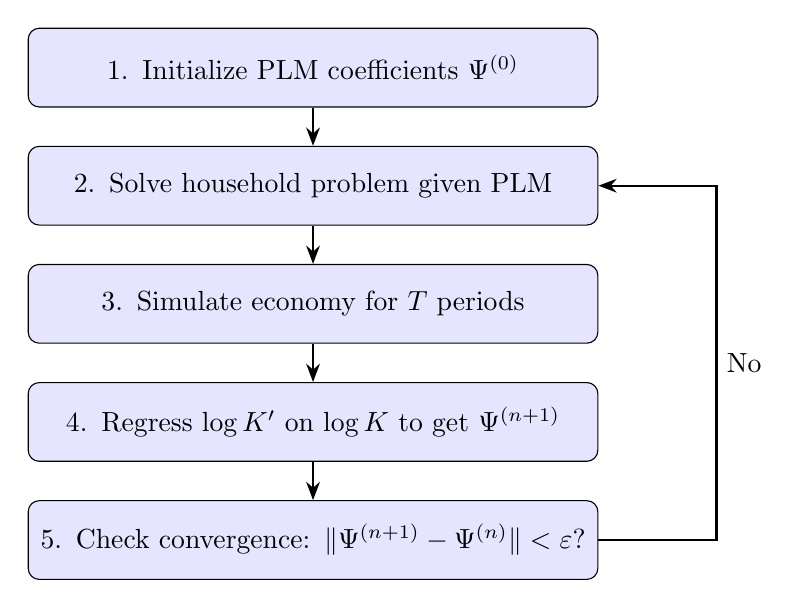
\begin{tikzpicture}[node distance=1.5cm, auto,
    block/.style={rectangle, draw, fill=blue!10, text width=7cm, text centered, rounded corners, minimum height=1cm},
    arrow/.style={-Stealth, thick}]
    
    \node[block] (init) {1. Initialize PLM coefficients $\Psi^{(0)}$};
    \node[block, below of=init] (solve) {2. Solve household problem given PLM};
    \node[block, below of=solve] (simulate) {3. Simulate economy for $T$ periods};
    \node[block, below of=simulate] (regress) {4. Regress $\log K'$ on $\log K$ to get $\Psi^{(n+1)}$};
    \node[block, below of=regress] (check) {5. Check convergence: $\|\Psi^{(n+1)} - \Psi^{(n)}\| < \varepsilon$?};
    
    \draw[arrow] (init) -- (solve);
    \draw[arrow] (solve) -- (simulate);
    \draw[arrow] (simulate) -- (regress);
    \draw[arrow] (regress) -- (check);
    \draw[arrow] (check.east) -- ++(1.5,0) |- node[near start, right] {No} (solve.east);
  \end{tikzpicture}
  \end{center}
\end{frame}

\begin{frame}{Step 1: Initialize PLM}
  \begin{itemize}
      \item Set initial guess for PLM coefficients:
      \[
      \Psi^{(0)} = (a_0^{(0)}, a_1^{(0)}, b_0^{(0)}, b_1^{(0)})
      \]
      \item Common starting point:
      \begin{itemize}
          \item $a_1^{(0)} = b_1^{(0)} \approx 0.99$ (high persistence)
          \item $a_0^{(0)}, b_0^{(0)}$ chosen so steady-state $K$ is consistent
      \end{itemize}
      \item Or use steady-state Aiyagari model as initial guess
  \end{itemize}
\end{frame}

\begin{frame}{Step 2: Solve Household Problem}
  \small
  Given PLM $\Psi$, solve the Bellman equation:
  \[
  \tilde{V}(a, \epsilon; z, K) = \max_{a' \geq \underline{a}} \left\{ u(c) + \beta \sum_{z', \epsilon'} \pi(z', \epsilon' | z, \epsilon) \tilde{V}(a', \epsilon'; z', K') \right\}
  \]
  where:
  \begin{align*}
  c &= (1 + r(z, K) - \delta) a + y(\epsilon, w(z, K)) - a' \\
  K' &= H(z, K; \Psi) \quad \text{(from PLM)}
  \end{align*}
  
  Solution methods:
  \begin{itemize}
      \item Value function iteration on grid
      \item Endogenous grid method (faster)
      \item Policy function iteration
  \end{itemize}
\end{frame}

\begin{frame}{Step 3: Simulate the Economy}
  \begin{itemize}
      \item Track $I$ agents for $T$ periods (e.g., $I = 10,000$, $T = 11,000$)
      \item Initialize: draw $(a_0^i, \epsilon_0^i)$ from ergodic distribution
      \item For each period $t$:
      \begin{enumerate}
          \item Compute aggregate capital: $K_t = \frac{1}{I} \sum_{i=1}^{I} a_t^i$
          \item Draw aggregate shock $z_{t+1}$ from Markov chain
          \item For each agent $i$:
          \begin{itemize}
              \item Draw $\epsilon_{t+1}^i$ from $\pi(\cdot | \epsilon_t^i, z_t, z_{t+1})$
              \item Compute $a_{t+1}^i = \tilde{g}(a_t^i, \epsilon_t^i; z_t, K_t)$
          \end{itemize}
      \end{enumerate}
      \item Discard first $T_0$ periods (burn-in, e.g., $T_0 = 1,000$)
  \end{itemize}
\end{frame}

\begin{frame}{Step 4: Update PLM via Regression}
  \begin{itemize}
      \item From simulation, obtain time series $\{K_t, z_t\}_{t=T_0}^{T}$
      \item Run OLS regressions separately for each $z$:
      \[
      \log K_{t+1} = a_0 + a_1 \log K_t + \varepsilon_t \quad \text{for } t : z_t = z_g
      \]
      \[
      \log K_{t+1} = b_0 + b_1 \log K_t + \varepsilon_t \quad \text{for } t : z_t = z_b
      \]
      \item New PLM coefficients: $\Psi^{(n+1)} = (\hat{a}_0, \hat{a}_1, \hat{b}_0, \hat{b}_1)$
      \item Check $R^2$ for forecast quality (should be $> 0.9999$)
  \end{itemize}
\end{frame}

\begin{frame}{Step 5: Check Convergence}
  \begin{itemize}
      \item Convergence criterion:
      \[
      \|\Psi^{(n+1)} - \Psi^{(n)}\| < \varepsilon
      \]
      \item Typically $\varepsilon = 10^{-4}$ or smaller
      \item If not converged:
      \begin{itemize}
          \item Update: $\Psi^{(n+1)} = \lambda \Psi^{(n+1)} + (1-\lambda) \Psi^{(n)}$
          \item Dampening factor $\lambda \in (0.3, 0.5)$ for stability
          \item Return to Step 2
      \end{itemize}
      \item If converged:
      \begin{itemize}
          \item Verify $R^2 > 0.9999$ for both regressions
          \item This validates the approximate equilibrium
      \end{itemize}
  \end{itemize}
\end{frame}

\begin{frame}{The Near-Aggregation Property}
  \begin{itemize}
      \item Surprising result: First moment ($\bar{K}$) is nearly sufficient
      \item $R^2 > 0.99999$ in original KS paper
      \item Intuition:
      \begin{itemize}
          \item Employed agents (high income) save similarly
          \item Unemployed agents (low income) dissave similarly
          \item Individual differences average out in aggregation
          \item Distribution shape matters little for aggregate $K'$
      \end{itemize}
      \item This is called approximate aggregation
      \item Does NOT always hold (e.g., with larger shocks or more nonlinearity)
  \end{itemize}
\end{frame}



\end{document}